%\subsection{数学理论}

\subsection{单纯形面}
\label{sec:simplicialSurface}
\begin{defn}
  令 $v_0,\ldots,v_d$是$\mathbb{R}^n$空间的$d+1$个仿射独立点,
  $d$是非负整数。
  定义\textbf{单形}$\sigma$是由点 $v_0,\ldots,v_d$张成的凸包,
  记做$[v_0,\ldots,v_d].$
  其中$v_0,\ldots,v_d$是$\sigma$的顶点,
  $d$是$\sigma$的维数,
  $\sigma$ 也称为 $d$-\textbf{单形}。
\end{defn}

\begin{defn}
  \label{defn:combinatorial}
  令 $\sigma= [v_0,\ldots,v_d]$是$\mathbb{R}^n$空间中的
  一个$d$-单形。
  $\sigma$的\textbf{面}是指由$\{v_0,\ldots,v_d\}$的一个子集张成的单形。
\end{defn}
\begin{defn}
  $\mathbb{R}^n$中的单纯复形${\cal K}$是$\mathbb{R}^n$中单形的有限集合,
  满足
  \begin{enumerate}
  \item 若$\sigma\in {\cal K}$, $\sigma$的面也属于${\cal K}$;
  \item 若$\sigma,\tau\in {\cal K}$,
    且$\tau\cap\sigma\neq
    \emptyset,$那么$\tau\cap\sigma$是$\sigma$和$\tau$的面。
  \end{enumerate}
\end{defn}

\begin{defn}
  ${\cal K}$的维数定义为
  \begin{equation}
    \dim({\cal K})=\max\{\dim(\sigma)\ \vert\ \sigma\in {\cal K}\}.
  \end{equation}
\end{defn}

\begin{defn}
  记$d$维的单纯复形${\cal K}$为$d$-\textbf{复形}。
  ${\cal K}$中所有单形上的点并称为${\cal K}$的底空间,
  记做$\lvert {\cal K}\rvert$
\end{defn}
  
\begin{defn}
  令${\cal K}$是$\mathbb{R}^n$中的一个单纯复形,
  对于${\cal K}$中的任意单形$\sigma$,
  $\sigma$的\textbf{star}和\textbf{link}分别定义如下:
  \begin{equation}
    \textmd{st}(\sigma,{\cal K})
    =\{\tau\in{\cal K}\vert\exists \eta \in {\cal K}
    \textmd{ 使得  }\sigma,\tau\textmd{ 都是 }\eta
        \textmd{ 的一个面 }\},
  \end{equation}
  以及
  \begin{equation}
      \textmd{lk}(\sigma,{\cal K})
    =\{\tau\in{\cal K}\vert \tau\in  \textmd{st}(\sigma,{\cal K})
    \textmd{ 且 }\tau,\sigma \textmd{ 没有共同的面} \}.
  \end{equation}
\end{defn}

\begin{defn}
  令${\cal K}$是$\mathbb{R}^n$中的一个2-复形。
  若每一个${\cal K}$中的1-单形正好是两个${\cal K}$中2-单形的面,
  而且每一个${\cal K}$中的0-单形的link同胚于单位圆$\mathbb{S}^1$,
  那么${\cal K}$是一个\textbf{单纯形面},$\lvert {\cal K}\rvert$
  是$\mathbb{R}^n$的一个拓扑曲面。
\end{defn}

\subsection{拓扑流形\cite{白正国2004黎曼几何初步}}
\label{sec:manifold}

\begin{defn}
  设$M$是一个Hausdorff拓扑空间,
  若对每一点$p\in M$,
  都有$p$的一个邻域$U$与$\mathbb{R}^n$的一个开集同胚,
  则称$M$为$n$\textbf{维拓扑流形}。
\end{defn}

\begin{nota}
  设$\varphi_U:U\rightarrow\varphi_U(U)\in \mathbb{R}^n$
  是上述定义中的一个同胚映射,
  则$(U,\varphi_U)$称为$M$的\textbf{坐标邻域}。
\end{nota}

\renewcommand{\theenumi}{\roman{enumi}}
\renewcommand{\labelenumi}{(\theenumi)}

\begin{defn}
  设$M$为$n$维拓扑流形,
  \begin{enumerate}
  \item $M$的一个坐标图开覆盖
    \begin{equation}
      \mathscr{U} = \{(U_{\alpha},\varphi_{\alpha})\ \vert\
      \alpha\in \mathscr{A},{\mathscr A}\textmd{ 为指标集},
      \ \bigcup_{\alpha\in {\mathscr A}}U_{\alpha}\ =\ M\}
    \end{equation}
    称为一个\textbf{坐标图册}。
  \item 若${\mathscr U}$中,对任何$\alpha,\beta\in \mathscr{A},$
    当$U_\alpha\cap U_\beta\neq \emptyset$时,
    \begin{displaymath}
      \varphi_\beta\circ \varphi_\alpha^{-1}:
      \varphi_\alpha(U_\alpha\cap U_\beta)\rightarrow
      \varphi_\beta(U_\alpha\cap U_\beta)
    \end{displaymath}
    为$C^k$映射,即坐标变换函数是$C^k$的,
    则称${\mathscr U}$为$C^k$\textbf{坐标图册},
    这时称$\mathscr{U}$中的坐标图是$C^k$\textbf{相容}的。
  \item 若${\mathscr U}$是最大的$C^k$坐标图册,
    即对于任意坐标邻域$(V,\varphi_V)$,
    当它与${\mathscr U}$坐标邻域$C^k$相容时,
    它也一定属于${\mathscr U}$,
    那么${\mathscr U}$称为$M$上的一个$C^k$\textbf{微分结构}。
    ${\mathscr U}$中的坐标领域称为$M$的\textbf{容许坐标邻域}。
  \end{enumerate}
\end{defn}

\begin{defn}
  设$M$是$m$维拓扑流形,
  $\mathscr{U}$是$M$上的一个$C^k$微分结构,
  则称$(M,\mathscr{U})$为$m$\textbf{维微分流形},
  简称$M$为\textbf{$m$维$C^k$流形}。
  特别,$m$维$C^{\infty}$流形也称为\textbf{光滑流形}。
\end{defn}

\begin{defn}
  $m$维$C^k$流形$M$上的一族$C^k$函数$\{f_i\ \vert\ i\in \mathbf{I}\}$,
  $\mathbf{I}$为正整数集,若具有如下性质:
  \begin{enumerate}
  \item $f_i(p)\geq 0, \forall p\in M$;
  \item $\sum_{i}f_i(p)=1$, 对任意点$p\in M$;
  \item $\{\textmd{supp}(f_i)\}$为$M$的局部有限的覆盖,
    则称$\{f_i\}$为$M$上的$C^k$\textbf{单位分解}。
  \end{enumerate}
\end{defn}

\begin{rem}
  单位分解联系了流形的局部性质和整体性质。
\end{rem}

\begin{defn}\label{defn:unitDecompose}
  设$\{A_\alpha\}$为$M$的一个开覆盖,
  $\{f_i\}$为$M$上的单位分解。
  若对于每个$i$, 存在一个$A_\alpha$使得
  $\textmd{supp}(f_i)\subset A_\alpha$,
  则称$\{f_i\}$为从属于$\{A_\alpha\}$的单位分解。
\end{defn}

\begin{thm}[单位分解定理]
  设$M$为具有可数基的$n$维$C^k$流形,
  $\{(U_i,\varphi_i;V_i)\}$为$M$的正则覆盖,
  则存在一个单位分解$\{f_i\}$,
  使得在$V_i$上$f_i> 0,$
  且$\textmd{supp}(f_i)\subset \varphi^{-1}_i(\ B_{3/4}^n(0)\ )$.
\end{thm}

\begin{thm}\label{thm:imbedding}
  设$M$是紧致$n$维微分流形,则存在一个正整数$m$
  及映射$f:M\rightarrow \mathbb{R}^m$,
  使得$f$为嵌入,
  从而$f(M)$是$\mathbb{R}^m$的正则子流形。
\end{thm}
\begin{pro}
  因为$M$紧致,故存在一个有限个坐标邻域组成的正则覆盖
  $\{(U_i,\varphi_i;V_i) \ \vert \ i=1,\ldots,k\}.$
  $\forall i,$ 由单位分解定理可知,
  存在函数$g_i:M\rightarrow \mathbb{R},$
  使得$g_i(M)\subset [0,1], V_i\subset \textmd{supp}(g_i)\subset U_i$,
  且在$V_i$上恒为1.
  令$f:M\rightarrow \mathbb{R}^{nk+k}$,
  使得
  \begin{equation}
    f(p) = (g_1\varphi_1(p),\cdots,g_k\varphi_k(p),g_1(p),\cdots,g_k(p)),
  \end{equation}
这里$g_i\varphi_i:M\rightarrow \mathbb{R}^n$定义如下:
\begin{equation}
  g_i\varphi_i(p)=
  \begin{cases}
    g_i(p)\varphi_i(p), &p \in U_i,\\
    0, &p \notin U_i.
  \end{cases}
\end{equation}
可以证明$f$是嵌入,且是单射。
\end{pro}

\subsection{Bernstein 基多项式}
\begin{nota}
  $d$\textbf{阶多项式空间}
  \begin{displaymath}
{\cal P}_d:=\left\{ p(x,y) = \sum_{0\leq i+j\leq d}c_{ij}x^iy^j\right\}.
  \end{displaymath}
\end{nota}

\begin{defn}
  给定整数$d>0$,和三角形$T=[q,r,s]\subset \mathbb{R}^2$
  相关\textbf{的$d$阶 Bernstein 基多项式}定义为
  \begin{displaymath}
    B^d_{ijk}(p):=\frac{d!}{i!j!k!}b^i_1b_2^jb_3^k,\quad i+j+k=d,
    \quad p=b_1q+b_2r+b_3s,
  \end{displaymath}
  $i,j,k$是非负整数, $b_1+b_2+b_3=1$是$p$关于三角形$[q,r,s]$的重心坐标。
\end{defn}

\begin{prop}
  Bernstein基多项式性质:
  \begin{enumerate}
  \item $ 0\leq B_{ijk}^d(p)\leq 1,\quad (p) \in T,$
  \item $ \sum_{i+j+k=d}B_{ijk}^d(p) \equiv 1,\quad (p)\in T.$
  \end{enumerate}
\end{prop}

\begin{lem}
  多项式 $\left\{ B^d_{ijk}\right\}$线性独立,
  且构成$d$次多项式${\cal P}_d$线性空间的一组基,维数是
  $\binom{d+2}{2}$。
\end{lem}

\begin{defn}[Bézier曲面片或三角曲面片]
  定义$d$-阶多项式曲面$b:\mathbb{R}^2\rightarrow \mathbb{R}^3$,
  \begin{equation}
    b(p)=b(b_1q+b_2r+b_3s)
    = \sum_{i+j+k=d}b_{ijk}\cdot B_{ijk}(b_1,b_2,b_3).
  \end{equation}
\end{defn}
\begin{rem}
  三次三角曲面片控制网格点确定一个曲面片。
  \begin{figure}[H]
    \centering
    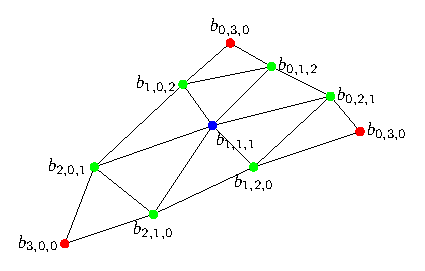
\includegraphics[width=0.3\linewidth]{tikz/controlNet}
    \label{fig:controlnet}
  \end{figure}
\end{rem}

\subsection{PN 三角曲面}
\label{sec:PNTriangle}

\begin{rem}
  从给定的单纯形面${\cal K}$构造PN 三角曲面。
  PN 三角曲面由一系列三次Bézier曲面片的组成,
  每个三角面片和${\cal K}$中一个特定的2-单形有关。
\end{rem}

\begin{rem}
  有很多种给定Bézier曲面片控制点的方式。
  其中有一种curved point-normal triangle(或者PN三角形)
  通过给定三角形三个顶点和顶点处单位法向量得到曲面片的控制点。
\end{rem}

\begin{defn}
  令$\sigma=[q_1,q_2,q_3]$是${\cal K}$中的任意2-单形,
  $\vec{n}_1,\vec{n}_2,\vec{n}_3$分别是${\cal K}$中包含$q_1,q_2,q_3$的
  2-单形的法向量平均。
  用$q_1,q_2,q_3,\vec{n}_1,\vec{n}_2,\vec{n}_3$定义三次Bézier曲面片
  的控制点
  $b_{3,0,0},b_{0,3,0},b_{0,0,3},b_{2,1,0},b_{1,2,0},b_{2,0,1},
  b_{0,2,1},b_{1,0,2},b_{0,1,2},b_{1,1,1}$如下:
  \begin{gather*}
        b_{3,0,0}=q_1,\quad b_{0,3,0}= q_2, \quad b_{0,0,3}=q_3,\\
        b_{2,1,0}=\frac{1}{3}(2q_1+q_2-c_{12}\vec{n}_1),\quad
        b_{1,2,0}=\frac{1}{3}(q_1+2q_2-c_{21}\vec{n}_2),\quad
        b_{0,2,1}=\frac{1}{3}(2q_2+q_3-c_{23}\vec{n}_2),\\
        b_{0,1,2}=\frac{1}{3}(q_2+2q_3-c_{32}\vec{n}_3),\quad
        b_{1,0,2}=\frac{1}{3}(q_1+2q_3-c_{31}\vec{n}_3),\quad
        b_{2,0,1}=\frac{1}{3}(2q_1+q_3-c_{13}\vec{n}_1),\\
      \end{gather*}
      其中$c_{ij}=(q_j-q_i)\cdot \vec{n}_i,\forall
      i,j\in\{1,2,3\},i\neq j$
      且
      \begin{displaymath}
        b_{1,1,1}=e+\frac{1}{2}(e-l),
      \end{displaymath}
      其中$e=\frac{1}{6}(b_{2,1,0}+b_{1,2,0}+b_{2,0,1}
      +b_{0,2,1}+b_{1,0,2}+b_{0,1,2})$且
      $l=\frac{1}{3}(q_1+q_2+q_3)$.
      定义2-单形$\sigma$上的PN三角形曲面片
      $b_\sigma:\mathbb{R}^2\rightarrow\mathbb{R}^3$
      为如下的三次Bézier曲面片
      \begin{equation}
        b_\sigma(p)=b_\sigma(\lambda q+\nu r+\mu s)=
        \sum_{i+j+k=3}b_{ijk}B_{ijk}(\lambda,\nu,\mu),
      \end{equation}
      其中,$\lambda,\nu,\mu$是点$p\in\mathbb{R}^2$关于三角形$T=[q,r,s]$
      的重心坐标。
      则集合$\bigcup_{\sigma\in {\cal K}}b_\sigma(T)$
      是关于${\cal K}$的PN三角曲面。
\end{defn}

\begin{rem}
  PN三角曲面是$C^0$连续的。
\end{rem}

%%% Local Variables:
%%% mode: latex
%%% TeX-master: "../3DmarsMathDoc"
%%% End:
